\documentclass[a4paper, 10pt]{report}
\usepackage[a4paper, left=2cm, right=3cm, top=2cm, bottom=4cm]{geometry}
\usepackage{ngerman}
\usepackage[utf8]{inputenc}
\usepackage{ulem}
\usepackage{amsmath}
\usepackage{amsfonts}
\usepackage{amssymb}
\usepackage{graphicx}

\begin{document}
\begin{titlepage}
\centering

\includegraphics[scale=1]{FAU-nat-logo.png}\par
\vspace{2cm}
{\huge\bfseries Kostengünstig in den Weltraum\par}
\vspace{1cm}
{\Large Michael Banken, Veit Simoneit, Dominik Winkel\par}
\vspace{2cm}
{\Large Mathematische Modellierung WS17/18\par}
\vspace{0.5cm}
{Betreut von Herr Prof. Dr. Kräutle\par}
\vfill
{\Large \today\par}

\end{titlepage}

\tableofcontents


\chapter{Einleitung}


Die vorliegende Arbeit beschäftigt sich mit der Frage ob es kostengünstige Alternativen gibt zu Raketen und Spaceshuttles um in den Weltraum, bzw. eine stabile erdnahe Umlaufbahn zu erreichen.\\
\chapter{Was ist Weltraum?}

Definitionen:
Weltraum
geostationärer Orbit
...

\chapter{Turm vs. Aufzug?!?!?}


\chapter{Aufzug}

\section{Seil}

...
\section{Design}

Nachdem gezeigt worden ist, dass ein Seil ins Weltall stabil gespannt werden kann, widmen wir uns drei entscheidenden Designfragen: 
\begin{itemize}
\item Welches Material benötigen wir für das Seil?
\item Wie können wir Stabilität und Kosteneinsparungen vereinen?
\item Wie wird das Seil angebracht?
\end{itemize}

\section{Materialfrage}
\textsl{Geschrieben von Veit Simoneit}\\
Der limitierende Faktor beim Bau eines Aufzugs oder eines Turms bis zum geostationären Orbit ist das verwendete Material. Das Gewicht des Materials ist ein wichtiger Faktor, jedoch noch elementarer ist die spezifische Höhe des Materials. Spezifische Höhe, auch ''self support length'' genannt ist die maximale Länge eines Pfeilers aus einem spezfischen Material, der nur an der Spitze befestigt ist und der sein Eigengewicht tragen kann.\cite{wiki:Specific_strength}

Ohne Beschränkung der Allgemeinheit nehmen wir für die spezifische Höhe überall am Seil die gleiche Gravitation von $g_0 = 9,80665 m/s^2$ an.
Betrachten wir im Vergleich drei Materialien: Stahl, Kevlar und Carbon Nano Tubes. \cite[vergleiche]{ED00}
\subsection{Stahl}
Das klassische Baumaterial um Wolkenkratzer überall auf der Welt zu bauen: Stahl. Da Stahl per se kein homogenes Material sein muss, betrachten wir die physikalischen Werte für stainless steel ohne die allgemeine Gültigkeit zu verlieren. Die Dichte von Stahl wird angegeben mit $\varrho_S = 7850 kg/m^3$ \cite[Vgl.]{PE75}. Die Zugfestigkeit von Stahl beträgt $2*10^9 kg/m*s^2$ , was $2GPa$ entspricht. Man berechnet die spezifische Höhe nun durch die Formel 
\begin{equation}
\frac{Zugfestigkeit_{Stahl}}{Dichte_{Stahl}*g_0} = \frac{2*10^9}{7850*9,80665}
<=> 25 980 m \sim 26 km 
\end{equation}

Überprüfen wir kurz die Einheiten
\begin{equation}
\frac{\frac{kg}{m*s^2}}{\frac{kg}{m^3}*\frac{m^2}{s^2}}= \frac{\frac{kg}{m*s^2}}{\frac{kg*m^2}{m^3*s^2}} = \frac{1}{\frac{1}{m}} = m
\end{equation}
Bei einer Seildicke von $2 cm$ im Durchmesser und einer Länge von $144.000 km$ bedeutet dies eine Gesamtmasse von $\sim 355.000 t$.\cite{PE75}
Betrachten wir ein anderes Vergleichsmaterial.
\subsection{Kevlar}
Kevlar wird in modernen schusssicheren Westen verwendet, da es leichter als Stahl aber sehr stabil ist. Die Dichte von Kevlar wird mit $\varrho_K = 1440 kg/m^3$ angegeben und liegt somit bei ungefähr einem Sechstel der Dichte von Stahl. Die Zugfestigkeit von Kevlar liegt bei $3,6 GPa$ und ist folglich 1,8-mal zugfester als Stahl. Hieraus folgt die spezifische Höhe für Kevlar mit
\begin{equation}
\frac{Zugfestigkeit_{Kevlar}}{Dichte_{Kevlar}*g_0} = \frac{3,6*10^9}{1440*9,80665}
<=> 254 929 m \sim 254 km 
\end{equation}
Kevlar hat eine spezifische Höhe, die 10-mal so hoch ist wie die von Stahl, jedoch ist es bis jetzt nicht ausreichend um einen Space Elevator zu bauen. \cite{PE75}
\subsection{Carbon Nano Tubes}
Die Lösung der Materialfrage liegt in den \textsl{Carbon Nano Tubes}.
Bei einer theoretischen Zugfestigkeit von $30 - 130 GPa$ und einer Dichte von $\varrho_{CNT} = 1300 kg/m^3$ liegt die spezifische Höhe zwischen $2.350 - 10.000 km$. Laut Pearson ist der Bau eines Weltraumaufzugs, bzw. Turms vergleichbar mit dem Bau eines Turms von $4900 km$ in einem gleichmäßigen 1-g-Schwerefeld \cite{PE75}. Und genau diese Voraussetzung erfüllen die Carbon Nano Tubes.
\section{Tapering} 
\textsl{Geschrieben von Veit Simoneit}\\
Bereits im Vorfeld ist abzusehen, dass sehr viel Material benötigt wird um einen Aufzug, bzw. überhaupt erst ein Seil ins Weltall zu spannen. Es gilt die Materialmenge so optimal wie möglich zu gestalten. 
Die Zugspannung, die auf jedes Element des Seils wirkt, ist gegeben durch
\begin{equation}
Z(r) = \int_{R_E}^{r} A*\varrho*g_0*M_E*\frac{1}{\tilde{r}^2} - A*\varrho*\omega*\frac{ \tilde{r}}{r_{geo}^3} d\tilde{r}
\end{equation}
Hierbei ist $A$ der Durchmesser des Seils, $\varrho$ die Dichte des verwendeten Materials, $M_E$ ist die Masse der Erde, $R_E$ der Radius derselbigen, $\omega$ ist die Winkelgeschwindigkeit, und $r_{geo}$ der Radius des geostationären Orbits. Durch das Integral kann man für jeden Punkt entlang des Seils die entsprechende Zugkraft berechnen in Abhängigkeit davon, wie weit man von der Erdoberfläche entfernt ist.
Bisher sind wir davon ausgegangen ein Seil mit einheitlicher Dicke zu verwenden. Baachtet man jedoch, dass an unterschiedlichen Stellen im Seil eine unterschiedlich hohe Zugkraft herrscht, so kann man die Materialmenge der entsprechenden Zugkraft anpassen.
Wir setzen $A=\lambda*Z(r)$ und erhalten
\begin{equation}
Z(r) = \int_{R_E}^{r}\lambda*Z(r)*\varrho*g_0*M_E*\frac{1}{\tilde{r}^2} - \lambda*Z(r)*\varrho*\omega*\frac{ \tilde{r}}{r_{geo}^3} d\tilde{r}
\end{equation}
Differenziert man diese Gleichung folgt
\begin{equation}
Z'(r)= \lambda*Z(r)*\varrho*g_0*M_E*\frac{1}{r^2} - \lambda*Z(r)*\varrho*\omega*\frac{r}{r_{geo}^3}
\end{equation}
Dies ist eine nicht autonome homogene lineare Differentialgleichung 1. Ordnung mit dem Ergebnis
\begin{equation}
A(r)=A_{geo}*e^\frac{3r_0^2}{2*h*r_{geo}}*e^{\frac{-r_0}{h}*(\frac{r_0}{r}+\frac{r_0*r^2}{2r_{geo}^3}}
\end{equation}
Somit kann man das sogenannte Taper-Verhältnis berechnen
\begin{equation}
\frac{A}{A_0} = e^\frac{0,776*r_0}{h}.
\end{equation}
$h=\frac{\sigma}{\varrho*g_0}$ mit $\sigma$ ist die als konstant(!) gesetzte Belastung. Man erkennt mit zunehmendem $h$ nimmt das Taperverhältnis ab.
Aus Formel (4.5) folgt, dass die größte Zugkraft am geostationären Orbit auf das Seil wirkt. Dies kann auch daraus geschlussfolgert werden, dass an diesem Punkt zwei gleich große Kräfte in entgegengesetzte Richtungen wirken. Zum einen die Kraft des Seils, das Richtung Erde zieht und zum anderen der Teil des Seils, der vom geostationären Orbit aus von der Erde weg zeigt. Man beachte, dass der geostationäre Orbit genau der Punkt ist, an dem sich die Gravitationskraft der Erde und die Fliehkraft, die auf das Objekt wirkt gegenseitig aufheben, wäre eine Kraft größer, so würde sich das Objekt auf eine andere Umlaufbahn bewegen. Daraus folgt auch, dass die Kraft, die auf den geostationären Punkt wirkt, maximal ist. \\
In Abbildung 4.1 erkennt man, wie das Taperingverhältnis zunimmt bis zum geostationären Orbit und dann wieder abnimmt. Die Kurve ist nicht symmetrisch, da die Gravitation von der Erde weg mit einem anderen Faktor abnimmt, als sie zur Erde hin zunimmt.
\begin{figure}[h]
\centering
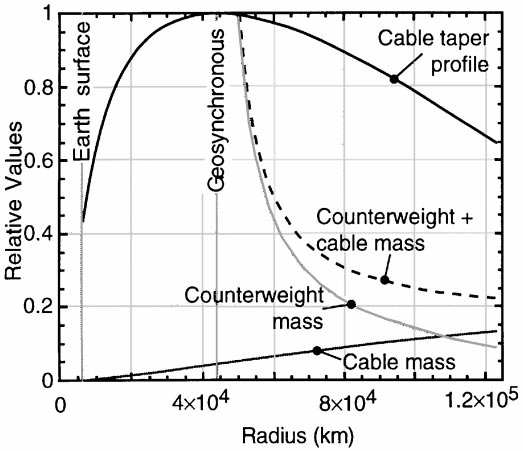
\includegraphics[scale=0.4]{Tapering.png} 
\caption{Kabel Taper Profil}
	\label{Abb:Tapering}
\end{figure}
\\
Vergleicht man die drei Materialien aus dem vorherigen Abschnitt bezüglich ihres Taper Verhältnisses am geostationären Punkt, so erhält man:

\begin{itemize}
\item Stahl: \ \ \ \ $\frac{A_{geo}}{A_0} = 5,8 *10^82$
\item Kevlar:\ \ \   $\frac{A_{geo}}{A_0} = 2,71 *10^8$
\item CNT: \ \ \ \ $\frac{A_{geo}}{A_0} = 1,62\ bis\ 8,2 $ 
\end{itemize}

Auf Grund der Größenordnung des Verhältnisses ist die einzige Lösung für die Materialwahl Carbon Nano Tubes, Stahl und Kevlar und andere Materialien haben ein zu großes Taperverhältnis.



\section{Deployment}



\bibliography{mybib}{}
\bibliographystyle{plain}

\appendix
\chapter{xxx}
\section{xxx}



\end{document}